\documentclass[a4paper, 12pt]{article}


\usepackage{amsmath}
\usepackage{multicol}
\usepackage{soulutf8}
\usepackage{float}
\usepackage{wrapfig}

\usepackage[russian]{babel}
\usepackage[T1]{fontenc}
\usepackage[utf8]{inputenc}

\usepackage{array}
\usepackage{tabularx}

\usepackage{caption}
\captionsetup[figure]{justification=raggedright, singlelinecheck=false}
\captionsetup[table]{justification=raggedleft, singlelinecheck=false}

\usepackage{titleps}


\usepackage{tikz}


\usepackage{geometry}
\geometry{left=15mm}
\geometry{right=15mm}
\geometry{top=10mm}
\geometry{bottom=20mm}

\setlength{\columnsep}{10mm}

\newpagestyle{myfooter1}{
    \setfoot{}{}{\thepage}
}

\newpagestyle{myfooter2}{
	\setfoot{3 Квант №6}{}{\thepage}
}



\setcounter{figure}{2}
\captionsetup[figure]{name=\bfseries \small Рис.}

\begin{document}
\setcounter{page}{63}
\pagestyle{myfooter1}

\begin{multicols}{2}
	Из подобия треугольников $SQA$ и $SPE$ имеем
	$$\frac{AQ}{PE} = \frac{SA}{SE},$$ 
	а из подобия треугольников  $SAC'$ и $SEC$
	
	$$\frac{SA}{SE} = \frac{AC'}{EC}$$
	
	Так как $AC' \perp SC$, то $AC’ < AC$, поэтому из (9) следует 
	$$\frac{SA}{SE} < \frac{AC}{EC}$$
	Из (8) и (10) получим 
	$$\frac{AQ}{PE} < \frac{AC}{EC} \text{ или } \frac{AQ}{AC} < \frac{PE}{EC}$$
	Треугольник $ABC$ правильный, поэтому 
	$$\frac{AQ}{AC} = \sin{30^\circ} = \frac12.$$
	Тогда из (11) следует 
	$$\sin{\angle PCE} = \frac{PE}{EC} > \frac12,$$
	то есть $\angle FCE$ больше $60^\circ$. Отсюда следует, что точки $A_1$ и $B_1$ лежат на отрезке $EF$, $Р$ --- середина $A_1B_1$ и $A_1B_1 < EF$.
	
	Теперь нетрудно сделать рисунок (рис. 3). Сторона основания $AB$ пирамиды  $SABC$
	
	\begin{figure}[H]
		\centering
		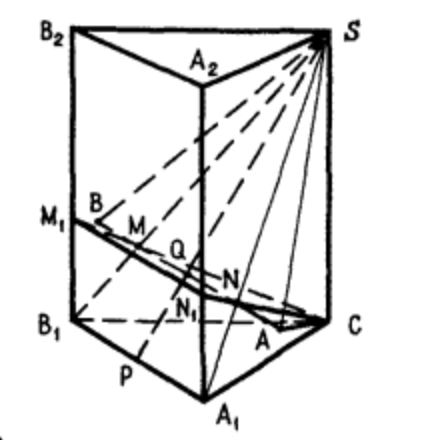
\includegraphics[width=.4\linewidth]{Image3.jpg}
		\caption{}
	\end{figure}
	
	пересекается с гранями призмы $A_1A_2SC$ и $B_1B_2SC$ в точках $M$  и $N$
	
	Обозначим $x = MN$, $a = AB$, $b = A_1B_1$, $h$ --- высота пирамиды. Найдем объемы пирамиды $SABC$ и ее части, лежащей внутри призмы:
	
	$$V_{SABC} = \frac16ah \cdot QC,$$,
	
	$$V_{SMNC} = \frac16hx \cdot QC,$$
	
	откуда
	
	$$\frac{V_{SABC}}{V_{SMNC}} = \frac{x}{a}$$
	
	\columnbreak
	\noindent
	Из подобия треугольников $MSN$ и $B_1SA_1$, находим
	$$\frac{x}{b} = \frac{SQ}{SP}$$
	Рассмотрим треугольник $SPC$ (рис. 4). Проведем прямую $QL \parallel PC$. Из подобия тре-
	\begin{figure}[H]
		\centering
		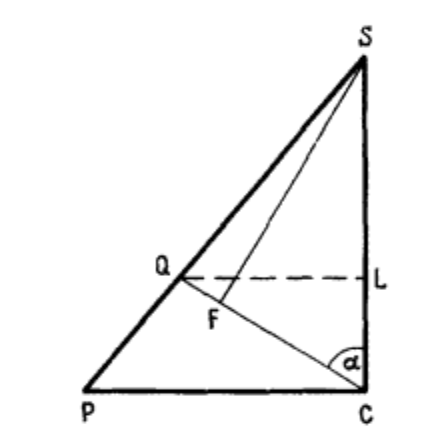
\includegraphics[width=.4\linewidth]{Image4.jpg}
		\caption{}
	\end{figure}
	\noindent
	угольников $SQL$ и $SPC$ имеем
	
	$$\frac{SQ}{SP} = \frac{QL}{PC}$$
	
	Далее,  $РС$ --- высота основания призмы, $PC = b\frac{\sqrt3}{2}$ и $QL = QC \cdot \sin{a}$.
	
	Угол $a$ --- это угол между ребром $SC$ и высотой $QC$ основания правильной пирамиды. Если $SF$ — высота пирамиды, то $FC = \frac{a\sqrt3}{2}$. По условию $SC = \frac{2}{\sqrt3}a$, откуда $\cos{a} = \frac12$, $a = 60^\circ$, и, следовательно, $QL = \frac{a\sqrt3}{2} \cdot \sin{60^\circ} = \frac{3a}{4}$
	
	Из (13) и (14) находим
	$$\frac{x}{b} = \frac{SQ}{SP} = \frac{QL}{PC} = \frac{\sqrt3a}{2b}$$,
	
	откуда $\frac{x}{a} = \frac{\sqrt2}{2}$, как следует из (12), дает искомое отношение объемов.
	
	\so{Ответ.} $\frac{\sqrt3}{2}$
	
	\centering\so{ Вариант 2}
	
	{\bfseries 1.} $63$ {\bfseries 2.} $x = \arcsin{\frac14} + 2\Pi k,$ $x = -\arcsin{\left( -\frac14 \right)}+ 2\Pi k.$
	
	{\bfseries 3.} $\frac{S_1S_3(S_1 + S_2)(S_2 + S_3)}{S_2(S_2^2 - S_1S_3)}$
\end{multicols}

\newpage
\setcounter{page}{17}
\pagestyle{myfooter2}
\vspace*{\fill}

\begin{multicols}{2}
Подставляя теперь значение $\delta E = F_T v \delta t$, получим
$$\delta v = -\frac{1}{m}F_T \delta t$$

Отсюда, считая изменения $\delta v$ и $\delta t$ малыми, получим выражение для ускорения спутника.

$$W = -\frac{1}{m}F_T$$

\columnbreak

\section*{\small\centering IV. Торможение в атмосфере}

Рассмотрим, что происходит при торможении спутника в земной атмосфере. В этом случае возмущающая (тормозящая) сила направлена против движения, то есть АЕ всегда имеет отрицательный знак. В соответствии с таблицей 1 большая полуось и период обращения будут постепенно убывать, следовательно, средняя

\end{multicols}

\begin{table}[!b]
	\caption{}
	\begin{tabular}{b{.45\textwidth} | b{.1\textwidth} | b{.2\textwidth} | b{.2\textwidth}}
	\hline
	Величина & Обозна- чение & Eсли $\delta E > 0$ (ускоряющая сила) & Eсли $\delta E < 0$ (тормозящая сила)\\\hline
	
	Радиус орбиты (большая полуось в случае движения по эллипсу) & $a$ & увеличивается & уменьшается\\
	
	Период обращения & $T$ & увеличивается & уменьшается\\
	
	Кинетическая энергия & $K$ & уменьшается & увеличивается\\
	
	Потенциальная энергия & $U$ & увеличивается & уменьшается\\
	
	Линейная скорость & $u$ & уменьшается & увеличивается\\ \hline
	\end{tabular}
\end{table}
\end{document}